
\section{Conclusão}

\begin{frame}
	\begin{center}
		Fórmulas com menos cláusulas produzem respostas mais rápido?
	\end{center}
	
	\begin{itemize}
		\pause\item Revisamos técnicas para reduzir o número de cláusulas \cite{plaisted1986structure,de1992optimality,jackson2004clause}.
		\pause\item Desenvolvemos um algoritmo de programação dinâmica para este problema.
		\pause\item Propomos experimentos para:
		\begin{itemize}
			\pause\item Verificar uma propriedade de optimalidade restrita do algoritmo proposto.
			\pause\item Comparar o algoritmo proposto com um outro.
			\pause\item Tentar responder à pergunta.
		\end{itemize}
	\end{itemize}
\end{frame}

\begin{frame}{Principais destaques}
	\begin{itemize}
		\item Tentar reduzir o tamanho de uma fórmula compensa.
		\pause\item Para este problema, DAGs são melhores que árvores.
		\pause\item É provável que nossa conjectura para árvores lineares esteja correta. \pause (trabalho futuro!)
		\pause\item Diferentes algoritmos de renomeamento levam vantagem em diferentes famílias de fórmulas. \pause Nas famílias \emph{SYJ206} e \emph{SYJ212}, o nosso gera muito menos claúsulas!
		\pause\item Considerando fórmulas parecidas, as com menos cláusulas tendem a dar resposta mais rápido.
	\end{itemize}
\end{frame}

\begin{frame}{Trabalhos futuros}
	\vspace{-.2cm}
	Para melhorar ainda mais o desempenho na etapa de busca:
	
	\pause
	\vspace{-.2cm}
	\begin{center}
		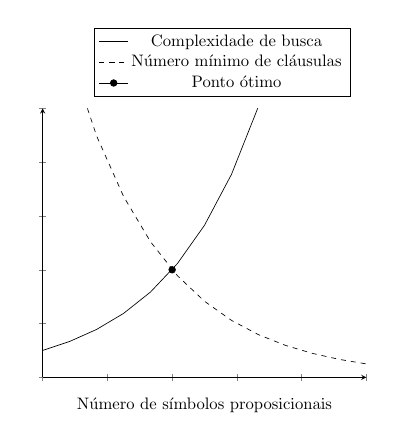
\begin{tikzpicture}[scale=.6]
		\begin{axis}[ymin=0,ymax=10,xmin=0,xlabel=Número de símbolos proposicionais,yticklabels={,,},xticklabels={,,},axis lines = left,legend entries={Complexidade de busca,Número mínimo de cláusulas,Ponto ótimo},legend style={at={(.95,1.3)}}]
		\addplot[mark=none]{2^x};
		\addplot[mark=none,dashed]{2^(4-x)};
		\addplot[mark=*] coordinates {(2,4)};;
		\end{axis}
		\end{tikzpicture}
	\end{center}
	
	\vspace{-.5cm}
	\pause Também reduz a complexidade do algoritmo proposto!
\end{frame}

\begin{frame}{Trabalhos futuros}
	\begin{footnotesize}
		\[
		f(i,j) =
		\begin{cases} 
		\hfill f(i-1,j-1) \cup \{\phi_i \}   \hfill & \text{ se } p(\phi,f(i-1,j-1) \cup \{\phi_i \}) < p(\phi,f(i-1,j)) \\
		\hfill f(i-1,j) \hfill & \text{ caso contrário} \\
		\end{cases}
		\]
	\end{footnotesize}
	
	\pause Adaptar para outras formas normais!
\end{frame}